% -----------------------------------------------
% Template for SMC 2010
% adapted from the template for ISMIR 2009
% -----------------------------------------------

\documentclass{article}
\usepackage{smc2010}
\usepackage{times}
\usepackage{ifpdf}
\usepackage[english]{babel}
\usepackage{amssymb,amsmath} 

\hyphenation{ba-sed gra-phic}

% -------------------- my commands -----------------
\newcommand{\emptyseg}		{\ensuremath{\oslash}}
\newcommand{\seg}[1]			{Seg(#1)}
\newcommand{\lra}				{$\leftrightarrow$}
\newcommand{\rshift}			{\hspace*{9mm}}
\newcommand{\sshift}			{\hspace*{4mm}}
\newcommand{\osc}[1]			{{\small \texttt{#1}}}




%user defined variables
\def\papertitle{Interlude - A Framework for Augmented Music Scores}

\def\finalversion{}
\ifdefined \finalversion
\def\paperauthors{Fober and al.}
\def\paperauthorA{D. Fober}
\def\paperauthorB{C. Daudin}
\def\paperauthorC{Y. Orlarey}
\def\paperauthorD{S. Letz}
\def\authors{\paperauthorA \quad \paperauthorB \quad \paperauthorC \quad \paperauthorD}

\def\chafo{chapuis07,Fober:07a}
\def\dau{daudin07}

\else
\def\paperauthors{Last name et al.}
\def\paperauthorA{First author}
\def\paperauthorB{Second author}
\def\paperauthorC{Third author}
\def\paperauthorD{}

\def\chafo{anon}
\def\dau{anon}
\fi

% adds the automatic
% Saves a lot of ouptut space in PDF... after conversion with the distiller
% Delete if you cannot get PS fonts working on your system.

% pdf-tex settings: detect automatically if run by latex or pdflatex
\newif\ifpdf
\ifx\pdfoutput\relax
\else
   \ifcase\pdfoutput
      \pdffalse
   \else
      \pdftrue
\fi

\ifpdf % compiling with pdflatex
  \usepackage[pdftex,
    pdftitle={\papertitle},
    pdfauthor={\paperauthorA, \paperauthorB, \paperauthorC, \paperauthorD},
    bookmarksnumbered, % use section numbers with bookmarks
    pdfstartview=XYZ % start with zoom=100% instead of full screen; especially useful if working with a big screen :-)
   ]{hyperref}
  %\pdfcompresslevel=9
  \usepackage[pdftex]{graphicx}
  \usepackage[figure,table]{hypcap}

  % put here are the names of the the PDF figures for the PDFlatex
  \global \def\fig1{figure.pdf}

\else % compiling with latex
  \usepackage[dvips]{epsfig,graphicx}
  \usepackage[dvips,
    bookmarksnumbered, % use section numbers with bookmarks
    pdfstartview=XYZ % start with zoom=100% instead of full screen
  ]{hyperref}
  % hyperrefs are active in the pdf file after conversion
  \usepackage[figure,table]{hypcap}
  %define the EPS figures here as PDFlatex does not accept them
  \global \def\fig1{figure.eps}

\fi

%setup the hyperref package - make the links black without a surrounding frame
\hypersetup{
    colorlinks,%
    citecolor=black,%
    filecolor=black,%
    linkcolor=black,%
    urlcolor=black
}


% Title.
% ------
\title{\textsc{\papertitle}}

% Single address
% To use with only one author or several with the same address
% ---------------
%\oneauthor
% {Names should be omitted for double-blind reviewing}
% {Affiliations should be omitted for double-blind reviewing}

%Two addresses
%--------------
% \twoauthors
%  {\paperauthorA} {School \\ Department}
%  {\paperauthorB} {Company \\ Address}

% Three addresses
% --------------

\ifdefined \finalversion
 \oneauthor
   {\authors} {Grame - Centre National de Cr\'eation Musicale \\ {\tt {\{fober,daudin,orlarey,letz\}@grame.fr}}}

\else
 \threeauthors
   {\paperauthorA} {Affiliation1 \\ {\tt \href{mailto:author1@smcnetwork.org}{author1@smcnetwork.org}}}
   {\paperauthorB} {\bf Retain these fake authors in\\\bf submission to preserve the formatting}
   {\paperauthorC} { Affiliation3 \\ {\tt \href{mailto:author3@smcnetwork.org}{author3@smcnetwork.org}}}
\fi

% ***************************************** the document starts here ***************
\begin{document}
%
\capstartfalse
\maketitle
\capstarttrue
%
\begin{abstract}
An \emph{Augmented Music Score} is a graphic space providing the representation, composition and manipulation of heterogeneous music objects (music scores but also images, text, signals...), both in the graphic and time domains. In addition, it supports the representation of the music performance, considered as a specific sound or gestural instance of the score. This paper presents the theoretical foundation of the augmented music score as well as an application - an augmented score viewer - that implements the proposed solutions.
\end{abstract}
%

\section{Introduction}\label{sec:introduction}

Music notation has a long history and evolved through ages. From the ancient neumes to the contemporary music notation, the western culture is rich of the many ways explored to represent the music. From symbolic or prescriptive notations to pure graphic representation, the music score has always been in constant interaction with the creative and artistic process. 

However, although the music representations have exploded with the advent of computer music \cite{dann93b,selfridge-field97,hewlett01}, the music score, intended to the performer, didn't evolved in proportion to the new music forms. In particular, there is a significant gap between interactive music and the static way it is generally notated: a performer has generally a traditional paper score, plus a computer screen displaying a rough number or letter to indicate the state of the interaction system. 
At the same time, we can observe the emergence of new needs in terms of music representation. 

In the domain of electro-acoustic music, analytic scores - music scores made \emph{a postériori} - like the "Portraits polychromes"\footnote{http://www.ina-entreprise.com/entreprise/activites/recherches-musicales/portraits-polychromes.html}, become common tools for the musicologists but have little support from the existing computer music software, apart the remarkable approach proposed for years by the Acousmograph \cite{ACOUSM04,ACOUSM91}. 

In the music pedagogy domain and based on a mirror metaphor, experiments have been made to extend the music score in order to provide feedback to students learning and practising a traditional music instrument \cite{Fober:04c,Fober:07b}. With this approach, an extended music score has been developed, supporting various annotations, including performance representations based on the audio signal, all in the context of a dynamic score layout. The limitations of the system rely mainly on a monophonic score centered approach and on a static design of the performance representation, making the system tricky to extend and to reuse.

New technologies allow now for real-time interaction and processing of musical, sound and gestural information. The Interlude project\footnote{http://interlude.ircam.fr} takes place in this domain and touches upon new digital paradigms for exploration and interaction of expressive movement with music. The present work on \emph{Augmented Music Scores} is part of this project and addresses interaction with symbolic content issues, while extending and generalizing previous music score extension approaches \cite{Fober:07b}. 

At the heart of the Augmented Music Score are the following main objectives:
\begin{itemize}
\item the score extension to arbitrary graphic objects: actually, we aim to consider arbitrary graphic objects (music scores but also images, text, signal representation...) as possible score candidates;

\item the expression of relations between graphic and time space: considering that time is a constant and common property of all musical objects, we give a time position and a time dimension to any score component, which also implies to make the temporal relations graphically visible;

\item the performance representation, gesture or audio based, with the aim to develop a system dynamically extensible.
\end{itemize}

None of the existing systems for music representation includes these kind of features: although generally extended to support contemporary music, tools like Lilypond \cite{lilypond03}, ENP \cite{KUUSK06}, NoteAbility \cite{Hamel98} or the Guido Engine \cite{Fober:04b} proposes a \emph{traditional} music score approach and are not suited to dynamic music notation.

Although the organization of the graphic space consistently to the time space \cite{bresson08}, or the synchronization of various medias \cite{baggi09b}, are among the current concerns, no formalism has been proposed to express relations between time and graphic space in a general music context.

Although tools for sound visualizations have been developed \cite{sonic06, ACOUSM04}, they are based on a fixed set of representations and don't support dynamic extensions. 

Synchronization of heterogeneous medias in the graphic domain raises issues related to non-linearity, non-con-tinuity, non-bijectivity. Based on previous experience, we propose to approach the problem using \emph{segmentation} and the description of relations between \emph{segments} - we will next use the term \emph{mappings} to refer to these relations.

The representation of the music performance, whether sound or gestural, is approached with a reverse perspective: the graphic representation of a signal is viewed as a \emph{graphic signal}, i.e. as a composite signal including all the information for the graphic rendering. This approach, which abstracts the representation calculation, results in an opened system, that can be dynamically extended.

We will first describe the theoretical foundations of the mappings and the context of use in the augmented music score framework. Next, we will explain how the system handles the performance signals to build \emph{graphic signals}. Finally, an augmented music score viewer is presented and particularly its control API, which is actually a set of OSC messages\cite{wright02}.


%------------------------------------------------------------
\section{Time and graphic relations}
%------------------------------------------------------------
We talk of \emph{time synchronization in the graphic domain} to refer to the graphic representation of the temporal relations between components of a score. Our previous experience in this domain \cite{Fober:04c,Fober:07b} led us to approach the question of these relations by the means of \emph{segmentation} and the description of relations between \emph{segments}. The term \emph{mappings} is used to refer to these relations.

The role of a \emph{mapping} is to make connections between the \emph{segments} of different resources, where a \emph{segment} is a contiguous zone of a resource. As previously mentioned, a resource can be an arbitrary object (music notation, images, text, signals...). The mappings are typically used to link graphic positions, music time and audio resources locations. For example, a mapping between an audio recording and a music score makes the connection between audio locations (expressed in frames) and the music time (expressed in quarter note divisions). A mapping between a music score and its graphic representation makes the connection between music time positions and graphic positions. Combining these mappings allows to make connections between all the time based resources.

The next sections describe the theoretical foundation for the notions of \emph{segment, segmentation} and \emph{mapping}. These foundations are independent of any implementation and of any resource specific information. They are followed by concrete use cases, implemented in the framework of the augmented score viewer.


%----------------------------------------------------------------
\subsection{Definitions}
%----------------------------------------------------------------
We will first introduce the notions of time and graphic segments. Next we will generalize these concrete definitions to an abstract, generic segment definition.

\subsubsection{Time segment}
%----------------------------------------------------------------

A time segment is defined as an interval
 $i=[t_0,t_1[$ such as $t_0 \leqslant t_1$.

An interval $i=[t_0,t_1[$ is said empty when $t_0 = t_1$. We will use \emptyseg\ to denote empty intervals.

Intersection of time  segments (figure \ref{fig:tsegment}) is the largest interval such as:
\[ \forall i_{m},\ \forall  i_{n}, 
\ i_{m} \cap i_{n}  := \{ j \ |\ j \in i_m \ \land\ j \in i_n \}
\]

\vspace{-4mm}
\begin{figure}[htbp]
\centerline{
	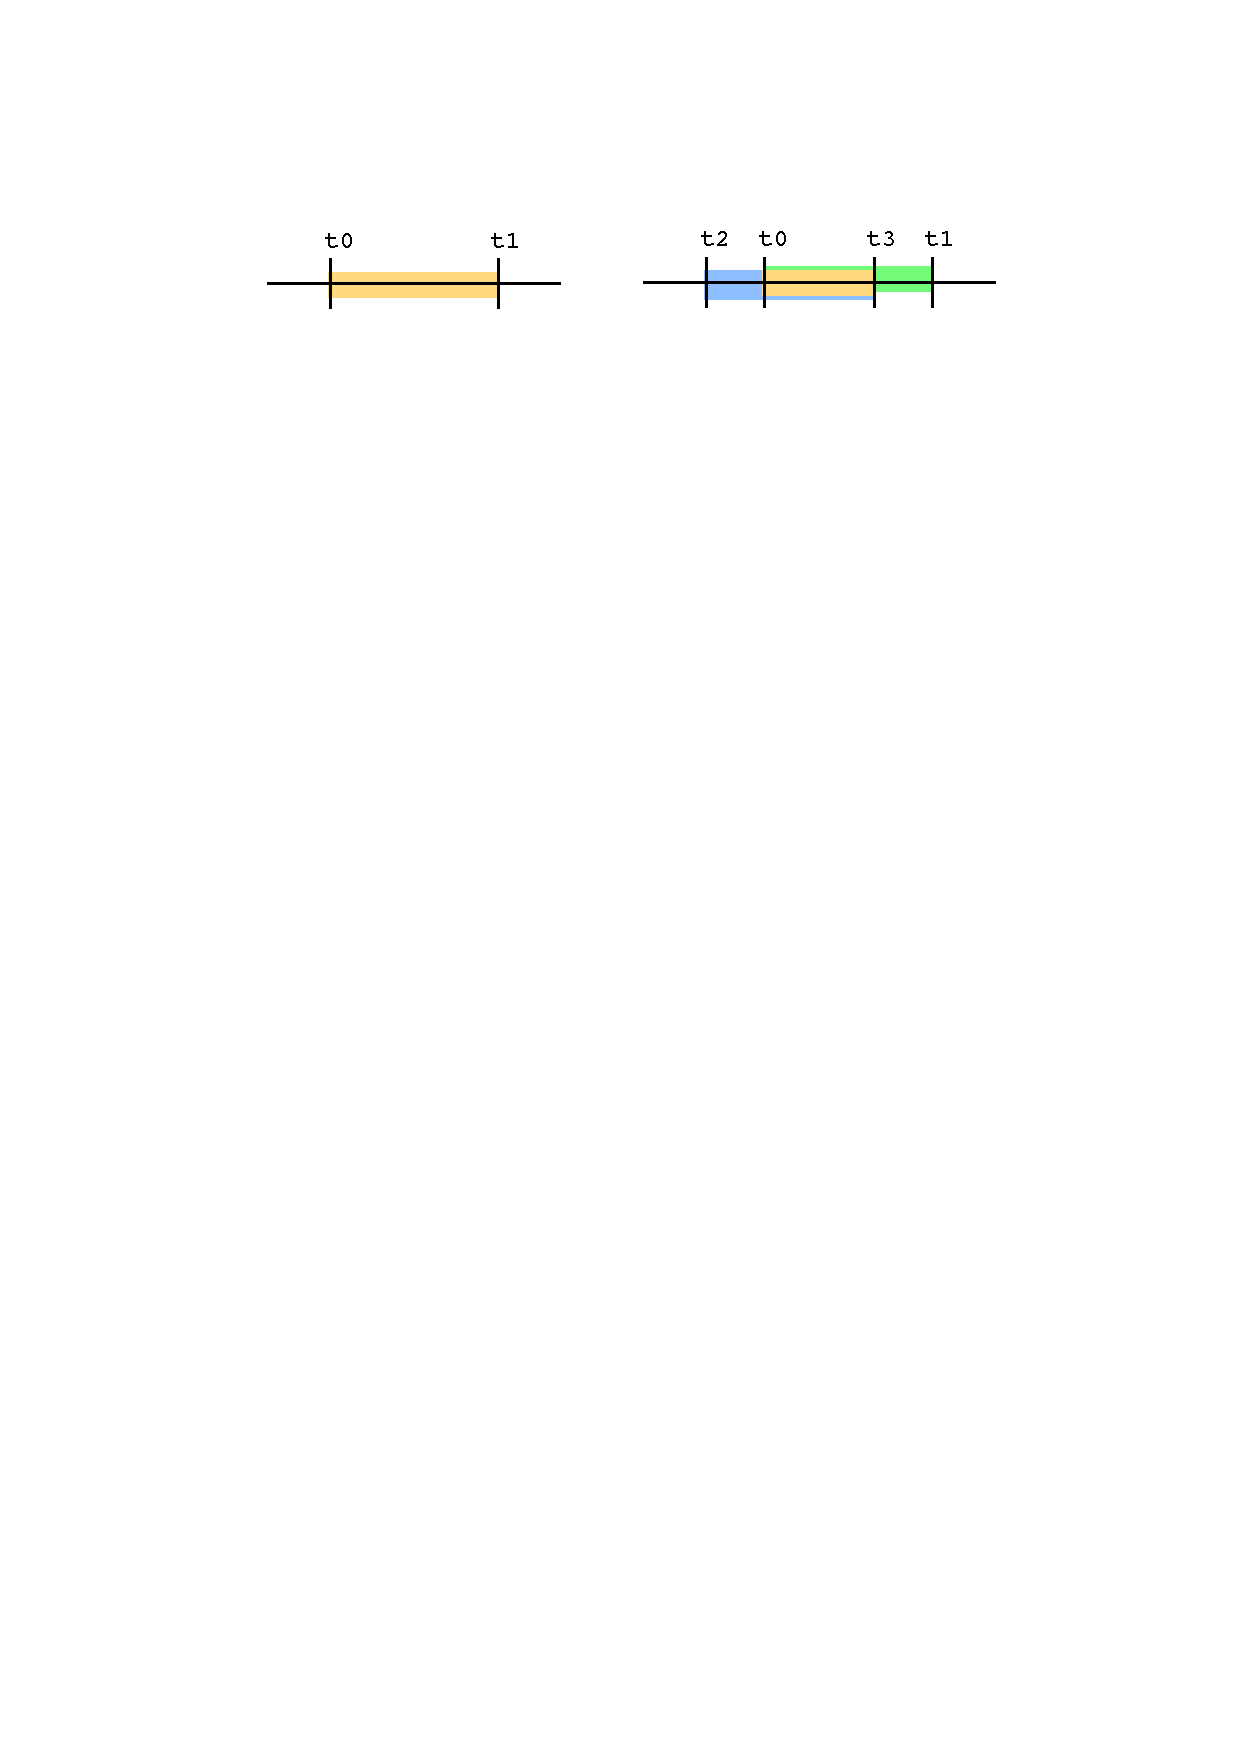
\includegraphics[width=0.8\columnwidth]{imgs/segments1D}}
\caption{From left to right: a time segment and time segments intersection.}
\label{fig:tsegment}
\end{figure}


%----------------------------------------------------------------
\subsubsection{Graphic segment}
%----------------------------------------------------------------
A graphic segment $g$ is defined as a rectangle given by two intervals $g=(i_x,i_y)$ where $i_x$ is an interval on the x-axis and $i_y$, on the y-axis.

A graphic segment $g=(i_x,i_y)$ is said empty when $i_x = \emptyseg $ or $i_y = \emptyseg $

The intersection operation $\cap$ between graphic segments (figure \ref{fig:gsegment}) is defined such as:
{\small
\[ \forall g=(i_x,i_y),\ \forall  g'=(i'_x,i'_y),\ 
g \cap g' = (i_x \cap i'_x, i_y \cap i'_y)
\]
}

\vspace{-4mm}
\begin{figure}[htbp]
\centerline{
	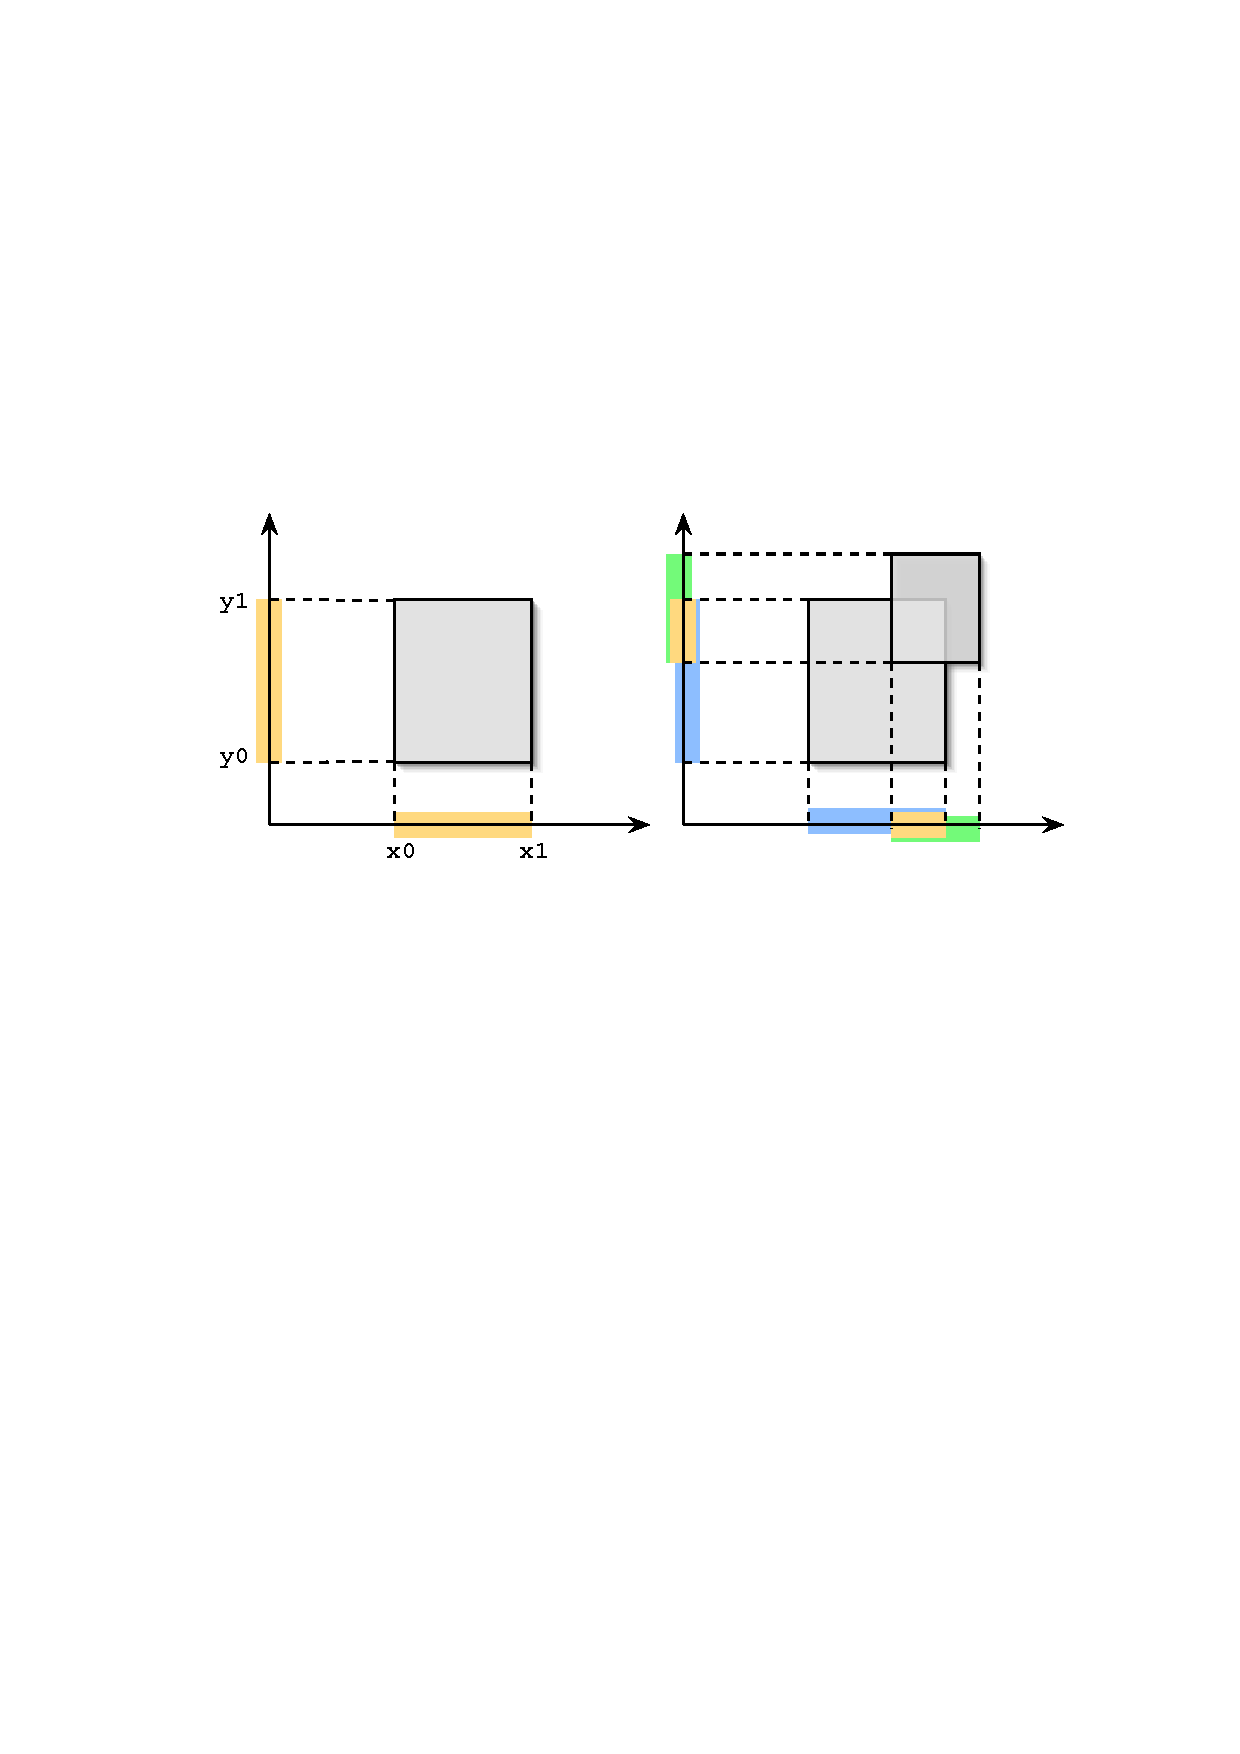
\includegraphics[width=0.8\columnwidth]{imgs/segments2D}}
\caption{From left to right: a graphic segment and graphic segments intersection.}
\label{fig:gsegment}
\end{figure}


%----------------------------------------------------------------
\subsection{Segment generalization}\label{subsec:generalseg}
%----------------------------------------------------------------
We will extend the definitions above to a general definition of a $n$-dimensional segment.
A $n$-dimensional segment is defined as a set of $n$ intervals $s^n=\{i_1,...,i_n\}$ where $i_j$ is an interval on the dimension $j$.

A segment $s^n$ is said empty when $\exists i \in s^n\ |\ i = \emptyseg $

Intersection between segments is defined as the set of their intervals intersection:
\begin{equation}
s_1^n \cap s_2^n = (i_1 \cap j_1, ... , i_n \cap j_n)
\end{equation}
where $s_1^n = (i_1, ... , i_n)$ et  $s_2^n = (j_1, ... , j_n)$


%----------------------------------------------------------------
\subsection{Resource segmentation}\label{subsec:resourceseg}
%----------------------------------------------------------------
A \emph{segment-able} resource $R$ is an $n$ dimensions resource defined by a segment $S^n$ of dimension $n$.\\
The segmentation of a resource $R$ is the set of segments
$\seg{R}=\{ s_1^n, ... s_i^n\}$ such as: \\
\begin{displaymath}
\begin{array}{rll}
\forall i, j \in \seg{R} & i \cap j =  \emptyseg  & $the segments are disjoint$ \\
\forall i \in \seg{R} & i \cap S^n = i & $segments are included in R$ \\
\end{array}
\end{displaymath}


%-------------------------------------------------------------
\subsection{Mapping}\label{subsec:mapping}

A \emph{mapping} is a relation between \emph{segmentations}.

For a mapping $M\subseteq \seg{R_{1}}\times \seg{R_{2}}$ we define two functions:
\begin{equation}
	M^{+}(i)=\{ i'\in \seg{R_{2}}\ |\ (i,i')\in M\}
\end{equation}
that gives the set of segments from $R_{2}$ associated to the segment $i$ from $R_{1}$; 
and the reverse function:
\begin{equation}
	M^{-}(i')=\{ i \in \seg{R_{1}}\ |\ (i,i')\in M\}
\end{equation}
that gives the set of segments from $R_{1}$ associated to the segment $i'$ from $R_{2}$.


These functions are defined for a set of segments as the union of each segment mapping:
\begin{equation}
	M^{+}(\{i_1, ...i_n\}) = \{ M^{+}(i_1) \cup M^{+}(i_2) ...  \cup M^{+}(i_n) \}
\end{equation}
and
\begin{equation}
	M^{-}(\{i_1, ...i_n\})=\{ M^{-}(i_1) \cup M^{-}(i_2) ...  \cup M^{-}(i_n) \}
\end{equation}

%----------------------------------------------------------------
\subsection{Mappings composition}\label{subsec:compmap}
Mappings composition is quite straightforward.\\
For a mapping $M_{1}\subseteq \seg{R_{1}}\times \seg{R_{2}}$ \\and a mapping $M_{2}\subseteq \seg{R_{2}}\times \seg{R_{3}}$, then :
\[ M_{1} \circ M_{2} \subseteq \seg{R_{1}}\times \seg{R_{3}} \]


%-------------------------------------------------------------
\subsection{Augmented Score segmentations and mappings}\label{sec:asm}

All the resources that are part of an augmented score have a graphic and a temporal dimension. Thus, they are \emph{segment-able} in the graphic and time spaces. Unless specified otherwise, time is referring to music time (i.e. metronomic time). 

In  addition, each resource type is \emph{segment-able} in its specific space: audio frames linear space for an audio signal, two dimensional space organized in lines/columns for text, etc.

\begin{table}[htdp]
\begin{center}
\begin{tabular}{|r|l|}
\hline
type & segmentations and mappings required \\
\hline
text		& \textit{graphic} \lra\ \textbf{text  \lra\ time} \\
score		& \textit{graphic \lra\ wrapped time} \lra\ \textit{time} \\
image		& \textit{graphic} \lra\ \textbf{pixel \lra\ time} \\
vectorial graphic	&  \textit{graphic} \lra\ \textbf{vectorial \lra\ time} \\
signal		&  \textit{graphic} \lra\ \textbf{frame \lra\ time} \\
\hline
\end{tabular}
\end{center}
\caption{Segmentations and mappings for each component type}
\label{maptable}
\end{table}

Table \ref{maptable} lists the segmentations and mappings used by the different component types. Mappings are indicated using arrows (\lra). Note that the arrows link segments of different types (the \emph{segment} qualifier is omitted). Segmentations and mappings in  \textit{italic} are automatically computed by the system, those in \textbf{bold} have to be provided externally. This typology could be extended to any kind of resource, provided that for any new type, a mapping exists to go from the graphic space to the time space. 

Note that an intermediate time segmentation, the \emph{wrapped time}, is necessary for music score in order to catch repeated sections and jumps (to sign, to coda, etc.).

Composition of these mappings is at the basis of the mechanisms to address and synchronize the components both in the graphic and time spaces.


%------------------------------------------------------------
\subsection{Synchronization examples}
%------------------------------------------------------------
Let's consider two score components $A$ and $B$ with their corresponding graphic and time segmentations: 
\vspace{1mm}\\
\rshift $\seg{A_g}$, $\seg{A_t}$, $\seg{B_g}$, $\seg{B_t}$. 
\vspace{1mm}\\
In addition, $B$ has an intermediate segmentation $\seg{B_l}$ expressed in the resource local space units (e.g. frames for an audio signal).
The mappings
\vspace{1mm}\\
\hspace*{5mm} $M_A \subseteq \seg{A_{g}}\times \seg{A_{t}}$ \\
and $M_B \subseteq \seg{B_{t}}\times \seg{B_{l}}$ 
\vspace{1mm}\\
give the correspondence between graphic and time space for $A$ and between time and local space for $B$.

When synchronizing objects and deciding on what position should be used as base position, we have introduced a master/slave relation between components: a slave is always constrained to its master space.

%------------------------------------------------------------
\subsubsection{Graphic alignment of time positions}

It corresponds typically to the alignment of a cursor on a score: the cursor indicates a time position but without temporal extension. 

Let's consider that $B$ is $A$ slave and we want to graphically align $B$ to $A$ at a time $t$. Let $s = [t_0, t_1[$ be the $A$ segment containing the time $t$. The corresponding graphic segment is:
\[
	M_A^{-}(s) =\{ g_i \in \seg{A_{g}}\ |\ (g,s)\in M_A\}
\]
When $M_A^{-}(s)$ contains a single segment, $B$ graphic position can be computed by simple linear interpolation i.e.:
\[
(x_B, y_B) = (g_{x0} + (g_{x1} - g_{x0}). \delta,\ g_{y0})
\]
where $g_{x0}$ and $g_{x1}$ are the graphic segment first and last $x$ coordinates and 
$\delta = (t - t_0) / (t_1 - t_0)$.

$y_B$ is arbitrary fixed to $g_{y0}$ but it is actually controlled by a synchronization mode (over, above, below).

When $s$ is mapped to several graphic segments, the operation can be repeated for each segment.


%------------------------------------------------------------
\subsubsection{Segments graphic alignment}

It corresponds typically to the alignment of a performance representation: the performance curve is made of segments (e.g. corresponding to notes) and each segment has to be aligned to the corresponding score location and duration.

The basic principle of segments alignment consists for each of the master graphic segment, to retrieve the corresponding slave segment expressed in the slave local coordinates and to render this slave segment in the space of the master graphic segment.
Provided that $\seg{A_t} = \seg{B_t}$, the operation may be viewed as the mapping composition 
\[
M_{A} \circ M_{B} \subseteq \seg{A_{g}}\times \seg{B_{l}}
\]
Figure \ref{fig:align} gives an example of different alignments obtained using different segmentations.
\begin{figure}[htbp]
\centerline{\framebox{
	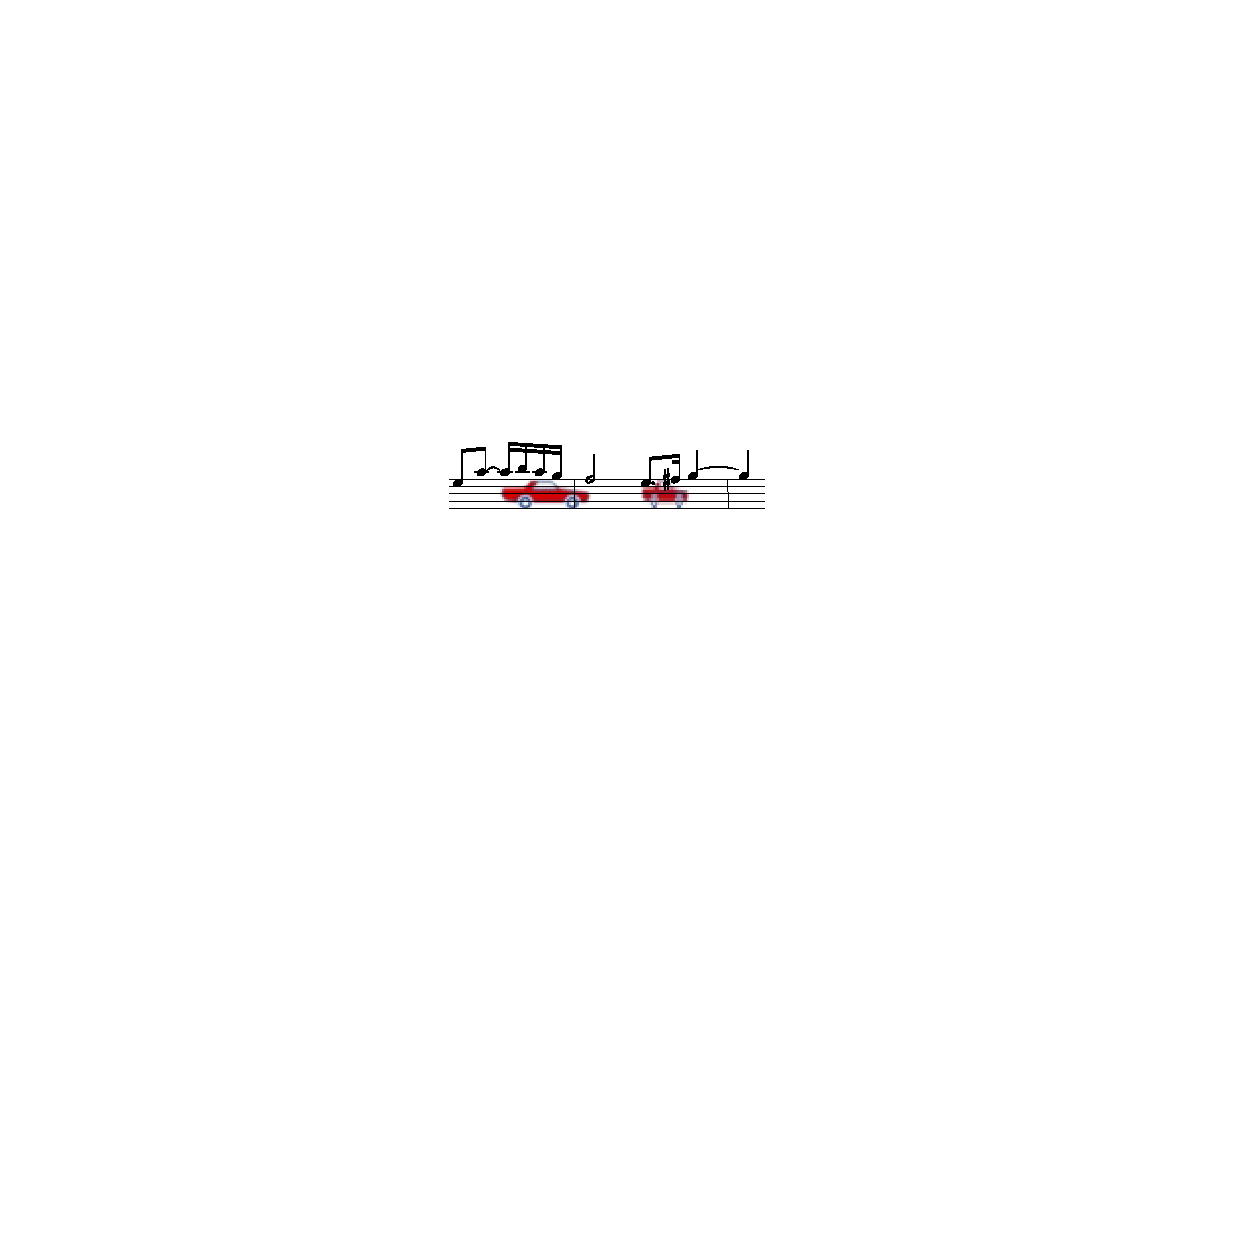
\includegraphics[width=0.7\columnwidth]{imgs/synccars}}}
\caption{The same car bitmap synchronized to different time positions. The image is made of a single graphic segment and has a quarter note duration. It is stretched to the corresponding score graphic segments.}
\label{fig:align}
\end{figure}


%------------------------------------------------------------
\section{Performance representation}

Work on the performance representation takes root in previous experiences about the visualization of music instrument playing, made in a pedagogic context \cite{Fober:07b}. Our previous approach was based on a graphic rendering engine, taking signals and a representation type as input, and producing the corresponding image.
The static embedding of the representation types in the rendering engine was one of the main limitations of the approach, implying to modify the engine for any new type.

In the context of the augmented score, our ambition was to develop a dynamically extensible system, avoiding this limitation. To do that, the graphic representation of a signal is viewed as a \emph{graphic signal}, i.e. as a composite signal including all the information required for its graphic rendering.

The resulting performance representation object is a \emph{first order} music score component: it has a date, a duration and thus can be synchronized to any other component.


%------------------------------------------------------------
\subsection{Graphic signals}

We define a graphic signal as a composite signal made of:
\begin{itemize}
\item a $y$ signal: the graphic $y$ coordinates
\item a $h$ signal: the graphic thickness at the $y$ position
\item a $c$ signal: the graphic color
\end{itemize}
To make simple, we assume that the color space addressed by $c$ has one dimension.
Figure \ref{fig:siggraph} gives an example of these parameters in the graphic space, at a time $t$. 

\begin{figure}[htbp]
\centerline{
	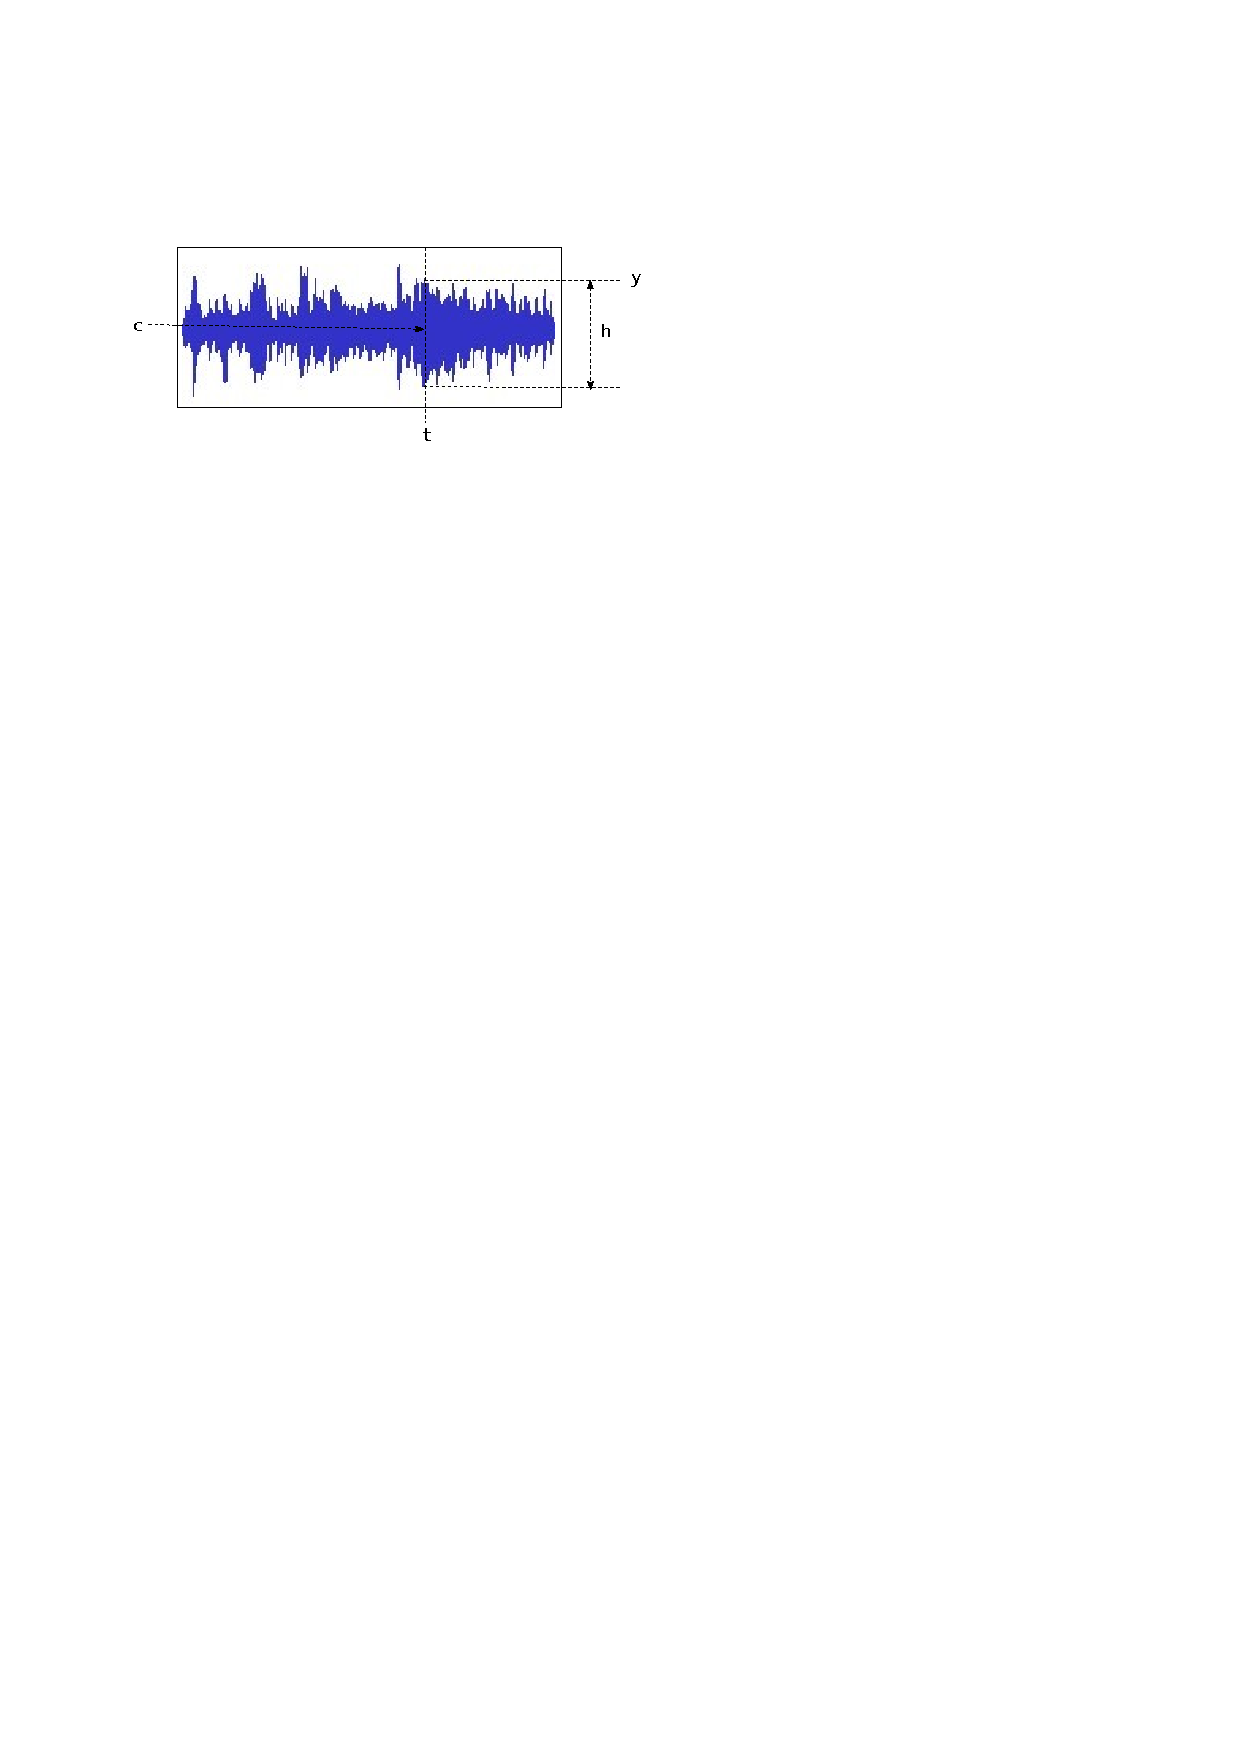
\includegraphics[width=0.90\columnwidth]{imgs/graph}}
\caption{Graphic signal parameters at a time $t$.}
\label{fig:siggraph}
\end{figure}

Now, let's consider a signal $S$ defined as a time function:
\[f(t)  : \mathbb{R} \rightarrow \mathbb{R}^3 =  (y, h, c)\ |\ y, h, c \in \mathbb{R} \]
then this signal may contain everything to be directly drawn i.e. without additional computation.

Such a system may also be viewed as an \emph{oscilloscope} taking the 3 graphic signal components as input.


%------------------------------------------------------------
\subsection{Signals composition}

In order to build composite signals to be used as graphic signals, we have introduced a signals parallelization operation.

Let's consider $\mathbb{S}$, the set of signals $s : \mathbb{N} \rightarrow \mathbb{R}$. \\
The \emph{parallel} operation '$/$' is defined as:
\begin{equation}
s_{1} / s_{2} / ... / s_{n} : \mathbb{S} \rightarrow \mathbb{S}^n\ |\ s_i \in \mathbb{S}
\end{equation}

The time function of a parallel signal $s^n \in \mathbb{S}^n$ is the parallelization of each signal's time function:
\begin{equation}
f(t) = (f_0(t), f_1(t), ... f_n(t))\ |\ f_i(t) :  \mathbb{N} \rightarrow \mathbb{R}
\end{equation}


%------------------------------------------------------------
\subsection{Parallel signals types}
To implement the system, we have defined several parallel signals types:
\begin{itemize}
	\item a \emph{color signal} type, based on the HSBA color model [hue, saturation, brigthness, transparency]:
	\[c ::= \overrightarrow{(h, s , b, a)} \ |\  h, s , b, a \in \mathbb{R}\] 
	\item a \emph{graphic signal} type that includes a $y$ signal, a thickness signal $th$,
	followed by the 4 components of the color signal:
	\[g ::= \overrightarrow{(y, th, h, s , b, a)} \ |\  y, th, h, s , b, a \in \mathbb{R}\]
	\item a \emph{parallel graphic signals} type to support several graphic signals in parallel: 
	\[g^n ::= \overrightarrow{g} \ |\  g \in \mathbb{R}^6\]
\end{itemize}


%------------------------------------------------------------
\subsection{Graphic signals examples}
In order to validate our model, we will describe several representation types that were statically implemented with the previous approach.
 
%-----------------------------------
\subsubsection{Pitch representation}
Represents notes pitches on the y-axis using the fundamental frequency (figure \ref{fig:pitch}).
\begin{figure}[htbp]
\centerline{
	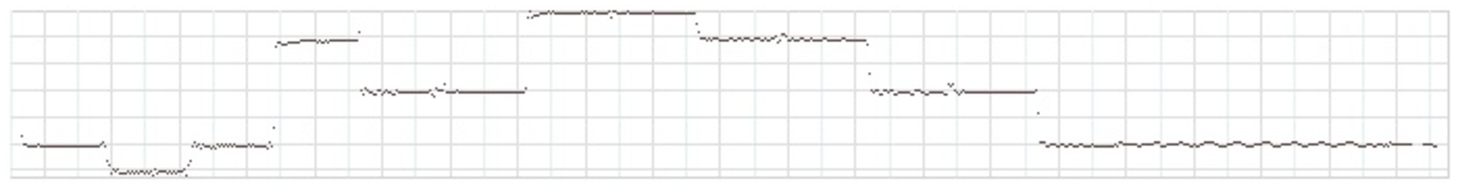
\includegraphics[width=0.99\columnwidth]{imgs/curves/pitch}}
\caption{Pitch representation.}
\label{fig:pitch}
\end{figure}

The corresponding graphic signal is expressed as:
\[ g = S_{f0}\ /\ k_t\ /\ k_c \]
where $S_{f0}$ : fundamental frequency \\
\rshift	 $k_t$ : a constant thickness signal \\
\rshift	 $k_c$ : a constant color signal 
 
%-----------------------------------
\subsubsection{Intonation representation}
Represents the difference between a fundamental frequency and a reference frequency
(figure \ref{fig:finepitch}).
\begin{figure}[h]
\centerline{
	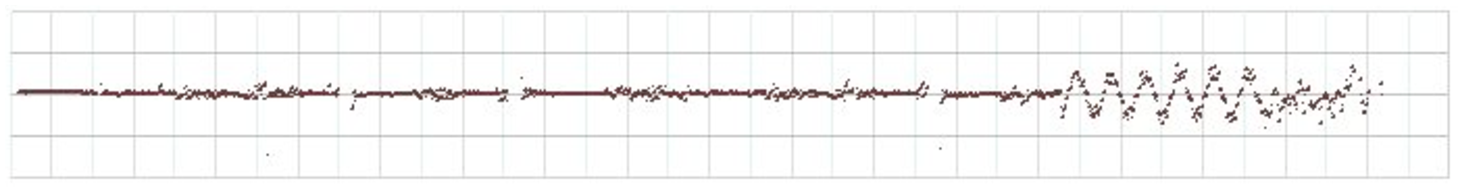
\includegraphics[width=0.99\columnwidth]{imgs/curves/finepitch}}
\caption{Intonation representation.}
\label{fig:finepitch}
\end{figure}

The corresponding graphic signal is expressed as:
\[ g = S_{f0}-S_{fr}\ /\ k_t\ /\ k_c \]
where $S_{f0}$ : fundamental frequency \\
\rshift	 $S_{fr}$ : reference frequency \\
\rshift	 $k_t$ : a constant thickness signal \\
\rshift	 $k_c$ : a constant color signal 
 
%-----------------------------------
\subsubsection{Articulations}
Makes use of the signal RMS values to control the graphic thickness
(figure \ref{fig:articulation}).
\begin{figure}[htbp]
\centerline{
	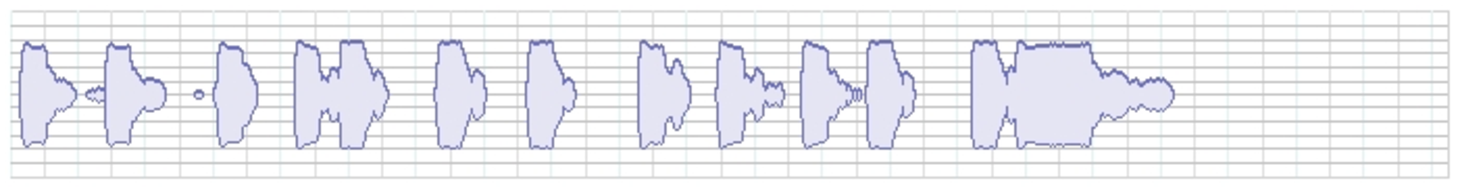
\includegraphics[width=0.99\columnwidth]{imgs/curves/articulation}}
\caption{Articulations.}
\label{fig:articulation}
\end{figure}

The corresponding graphic signal is expressed as:
\[ g = k_y\ /\ S_{rms}\ /\ k_c \]
where $k_y$ : signal $y$ constant \\
\rshift	 $S_{rms}$ : RMS signal \\
\rshift	 $k_c$ : a constant color signal 
 
%-----------------------------------
\subsubsection{Pitch and articulation combined}
\label{pitchart}
Makes use of the fundamental frequency and RMS values to draw articulations shifted by the pitches
(figure \ref{fig:pitchedarticulation}).
\begin{figure}[htbp]
\centerline{
	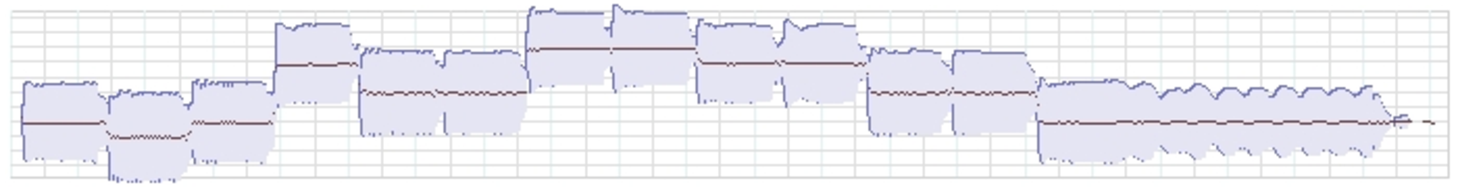
\includegraphics[width=0.99\columnwidth]{imgs/curves/pitchedarticulation}}
\caption{Pitch and articulation combined.}
\label{fig:pitchedarticulation}
\end{figure}

The corresponding graphic signal is expressed as:
\[ g = S_{f0}\ /\ S_{rms}\ /\ k_c \]
where $S_{f0}$ : fundamental frequency \\
\rshift	 $S_{rms}$ : RMS signal \\
\rshift	 $k_c$ : a constant color signal 
 
%-----------------------------------
\subsubsection{Pitch and harmonics combined}
Combines the fundamental frequency to the first harmonics RMS values
(figure \ref{fig:pitchedstackedharm}). Each harmonic has a different color.
\begin{figure}[htbp]
\centerline{
	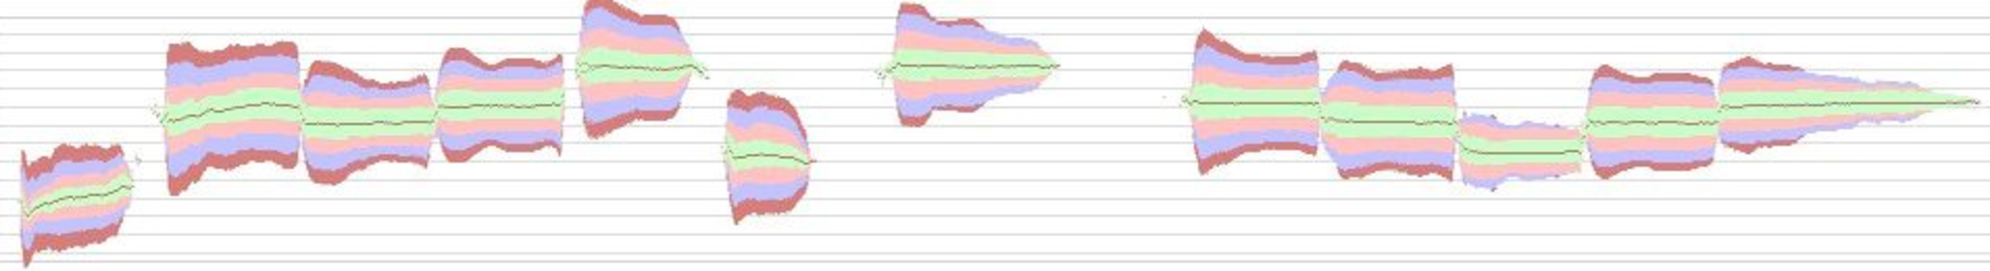
\includegraphics[width=0.99\columnwidth]{imgs/curves/pitchedstackedharm}}
\caption{Pitch and harmonics combined.}
\label{fig:pitchedstackedharm}
\end{figure}

We will describe the corresponding graphic signal in several steps. First, we build the fundamental frequency graphic as above (see section \ref{pitchart}) :
\[ g0 = S_{f0}\ /\ S_{rms0}\ /\ k_c0 \]
where $S_{f0}$ : fundamental frequency \\
\rshift	 $S_{rms0}$ : f0 RMS values \\
\rshift $k_c0$ : a constant color signal 

\vspace{2mm}
Next we build the graphic for the harmonic 1:
\[ g1 = S_{f0} \ /\ S_{rms1} + S_{rms0}\ /\ k_c1 \]
\rshift	 $S_{rms1}$ : harmonic 1 RMS values \\
\rshift $k_c1$ : a constant color signal

\vspace{2mm}
Next, the graphic for the harmonic 2:
\[ g2 = S_{f0} /\ S_{rms2} + S_{rms1}  + S_{rms0} \ /\ k_c2 \]
\rshift	 $S_{rms2}$ : harmonic 2 RMS values\\
\rshift $k_c2$ : a constant color signal 

\vspace{1mm}
etc.

\vspace{2mm}
And we finally combine them into a parallel graphic signal:
\[ g = g2 \ /\  g1 \ /\ g0 \]



%=============================================================
\section{The Augmented Music Score viewer}

The implementation takes the form of a C++ library - the Interlude library - as well as an augmented score viewer, build on top of this library. This viewer has no user interface since it has been primarily designed to be controlled via OSC messages i.e. using external applications like Max/MSP or Pure Data.

\subsection{Messages general format}

An Interlude OSC message is made of an OSC address, followed by a message string, followed by $0$ to $n$ parameters. The message string could be viewed as the method name of the object identified by the OSC address. 

The OSC address is a string or a regular expression matching several objects.
The OSC address space includes predefined static nodes:\\
\sshift \osc{/ITL} corresponds to the Interlude viewer application \\
\sshift \osc{/ITL/scene} corresponds to the rendering scene, actually the augmented score address.\\
The score components have addresses of the form: \\
\sshift \osc{/ITL/scene/anyname} where \osc{anyname} is an arbitrary user defined name.

The score components parameters can be addressed with messages strings like \osc{x}, \osc{y} or \osc{z} to control the $x$, $y$ or $z$ position. Table \ref{msgtable} gives the main message strings, supported by all the components. Almost these messages have a relative form e.g. \osc{dx} for a relative $x$ displacement.

\begin{table}[htdp]
\begin{center}
\begin{tabular}{|r|l|}
\hline
message strings & component parameters \\
\hline
\osc{x, y, z, scale, angle}		&  scale and position \\
\osc{date, duration, clock}		&  time management \\
\osc{color, hsb}		&  color management \\
\hline
\end{tabular}
\end{center}
\caption{The main messages, supported by all the score components.}
\label{msgtable}
\end{table}

The next sections present examples of OSC messages setting up a score including synchronized components. Note that the messages list corresponds strictly to the file format of a score. Note also that these examples are static while real-time interaction is always possible, for example to move objects in time by sending \osc{date} or \osc{clock} messages (similar to MIDI clocks).

\subsection{A simple cursor example}

This example shows a cursor synchronized to a graphic bitmap. Lines beginning with a '\#' are comments interleaved with the messages.
{\small \begin{verbatim}
# creates the score as an image
/ITL/scene/turenas set img "score.png"
# sets the image graphic to time mapping
/ITL/scene/turenas mapf "turenas.map"
# sets the score title and position
/ITL/scene/title set txt "Turenas - John..."
/ITL/scene/title x -0.36
/ITL/scene/title y -0.86
/ITL/scene/title scale 3.0
# creates a rectangle used as cursor
/ITL/scene/cursor set rect 0.004 0.217176
/ITL/scene/cursor z 0.5
/ITL/scene/cursor color 204 0 48 132
# synchronizes the cursor to the score
/ITL/scene/sync cursor turenas v
# moves the cursor in time
/ITL/scene/cursor date 123 4
\end{verbatim}

The mapping file \emph{turenas.map } describes the relation betwwen the image segments and the time. The image is segmented in 3 parts corresponding to each lines. For each line, the first segment applies to the graphic space (expressed in pixels intervals) and the second segment to the time space (expressed as rationals).

{\small \begin{verbatim}
( [27,780[ [15,193[ )   ( [0/4,225/4[ ) 
( [27,782[ [216,394[ )  ( [225/4,520/4[ )
( [27,511[ [417,594[ )  ( [520/4,594/4[ )
\end{verbatim}

The result is given by the figure \ref{fig:turenas}. The cursor is located to the image position corresponding to its date.

\begin{figure*}[htbp]
\centerline{\framebox{
	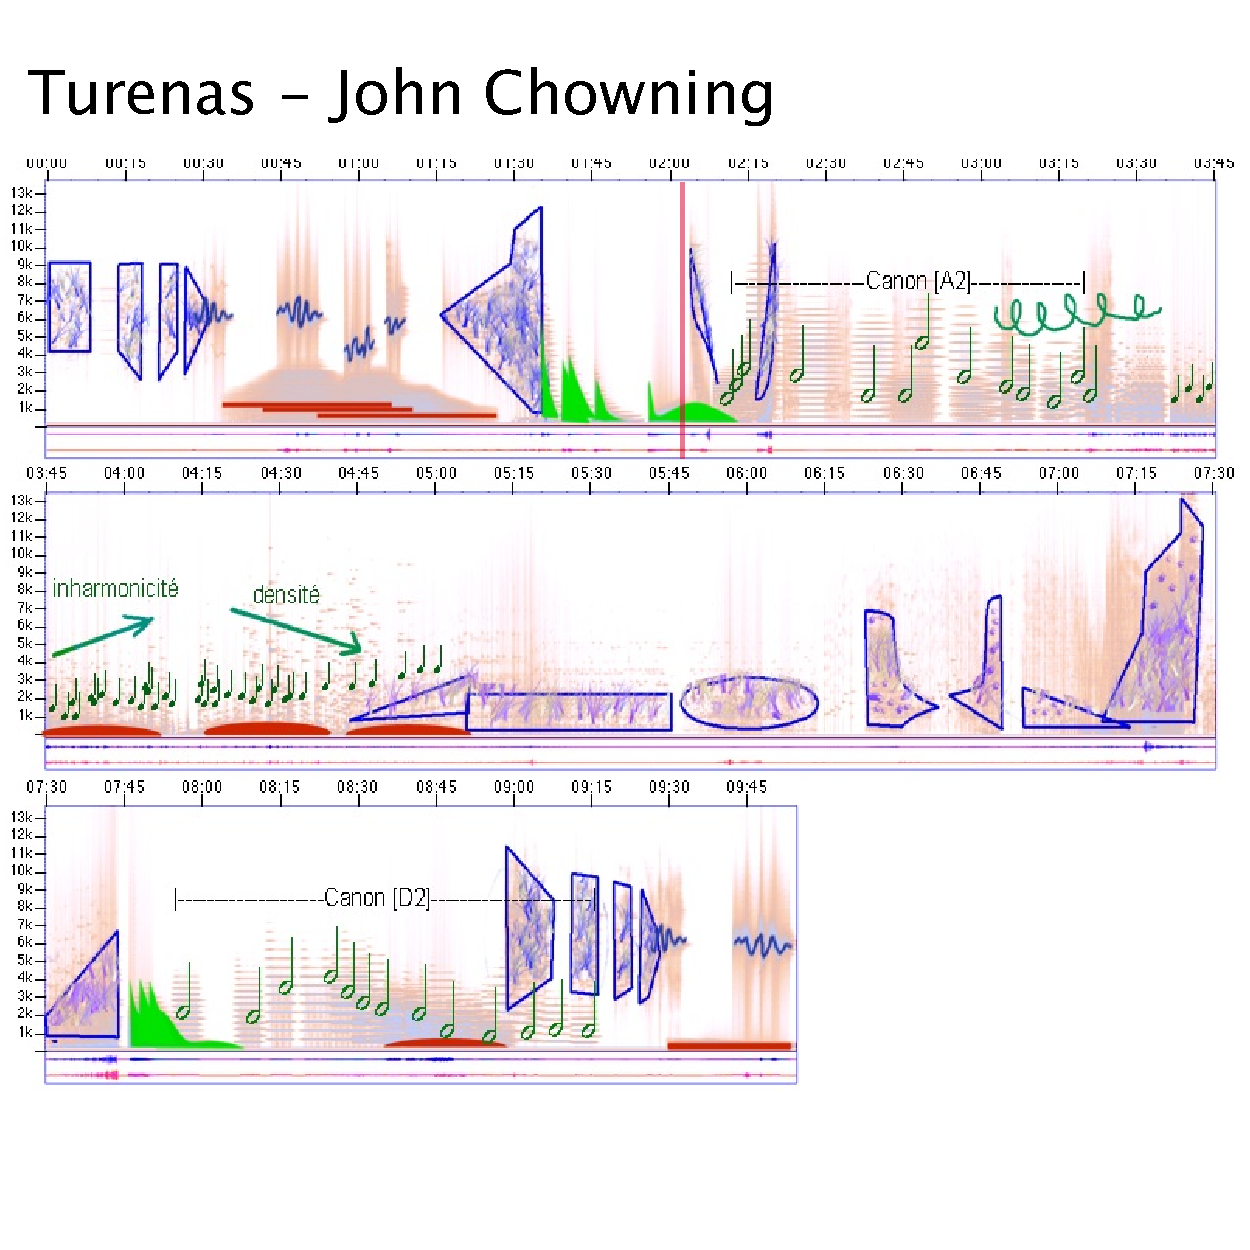
\includegraphics[width=1.6\columnwidth]{imgs/turenas}}}
\caption{Turenas score: analysis and graphic transcription by Laurent Pottier. The transcription is taken from the INA-GRM "Portraits polychromes" and reimplemented using the augmented score framework.}
\label{fig:turenas}
\end{figure*}


\subsection{Nested synchronization example}

This example uses 3 components; the first one is master of the second, which is master of the third one. 

{\small \begin{verbatim}
# creates a score using an image
/ITL/scene/score set img "score.jpg"
# sets the score graphic to time mapping 
/ITL/scene/score mapf "score.map"

# creates a text using a text file
/ITL/scene/text set txtf "comment.txt"
# changes the text scale
/ITL/scene/text scale 3.0
# and the text color
/ITL/scene/text color 0 0 240 255
# put the text in front
/ITL/scene/text z 0.5
# and sets the text to time mapping 
/ITL/scene/text mapf "comment.map"

# creates a ball as vectorial graphic
/ITL/scene/ball set ellipse 0.2 0.2
# puts it in front
/ITL/scene/ball z 0.4
# changes the ball color
/ITL/scene/ball color 250 50 0 255

# sets all the objects date
/ITL/scene/* date 4 1
# sets the text slave of the score
/ITL/scene/sync text score
# sets the ball slave of the text
/ITL/scene/sync ball text
\end{verbatim}
}Note the use of a wildcard in the OSC address to set all the objects date with a single message. 
The corresponding result is given by figure \ref{fig:scene}.

\begin{figure*}[htbp]
\centerline{\framebox{
	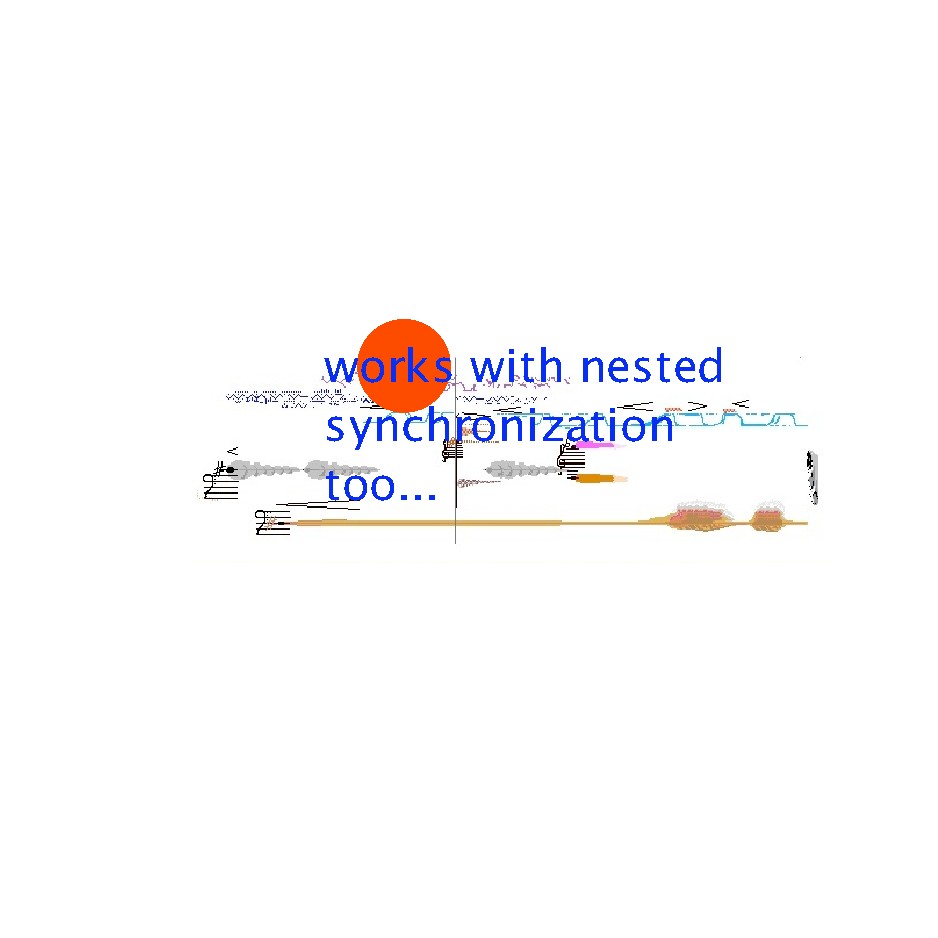
\includegraphics[width=1.6\columnwidth]{imgs/scene}}}
\caption{A score with nested synchronization. It includes a bitmap, text and a vectorial graphic. The text is synchronized to the bitmap and the circle to the text. When receiving time messages (e.g. clock), each object moves relatively to its master.}
\label{fig:scene}
\end{figure*}



\subsection{A signal synchronized to a score}

This example show a graphic signal synchronized to a GMN score. Note that a graphic signal is  a \emph{first order} music score component: it has a date and a duration and can be synchronized to any other object. 
{\small \begin{verbatim}
# declare a y signal with size 200
/ITL/scene/signal/y size 200 
# declare a thickness signal
/ITL/scene/signal/t size 200
# combines y and t + constant color signals
/ITL/scene/signal/sig set y t 0. 1. 1. 1.
# build the corresponding graphic signal
/ITL/scene/myGraph set graph sig
# set its date and duration
/ITL/scene/myGraph date 7 4
/ITL/scene/myGraph duration 2 4
# creates the score
/ITL/scene/score set gmnf "score.gmn"
# synchronize the graphic signal to the score
/ITL/scene/sync myGraph score h
\end{verbatim}

The corresponding result is given by figure \ref{fig:graph}. The signal can move and receive data in real-time. Note that the score graphic to time mapping is automatically computed by the system.

\begin{figure*}[htbp]
\centerline{\framebox{
	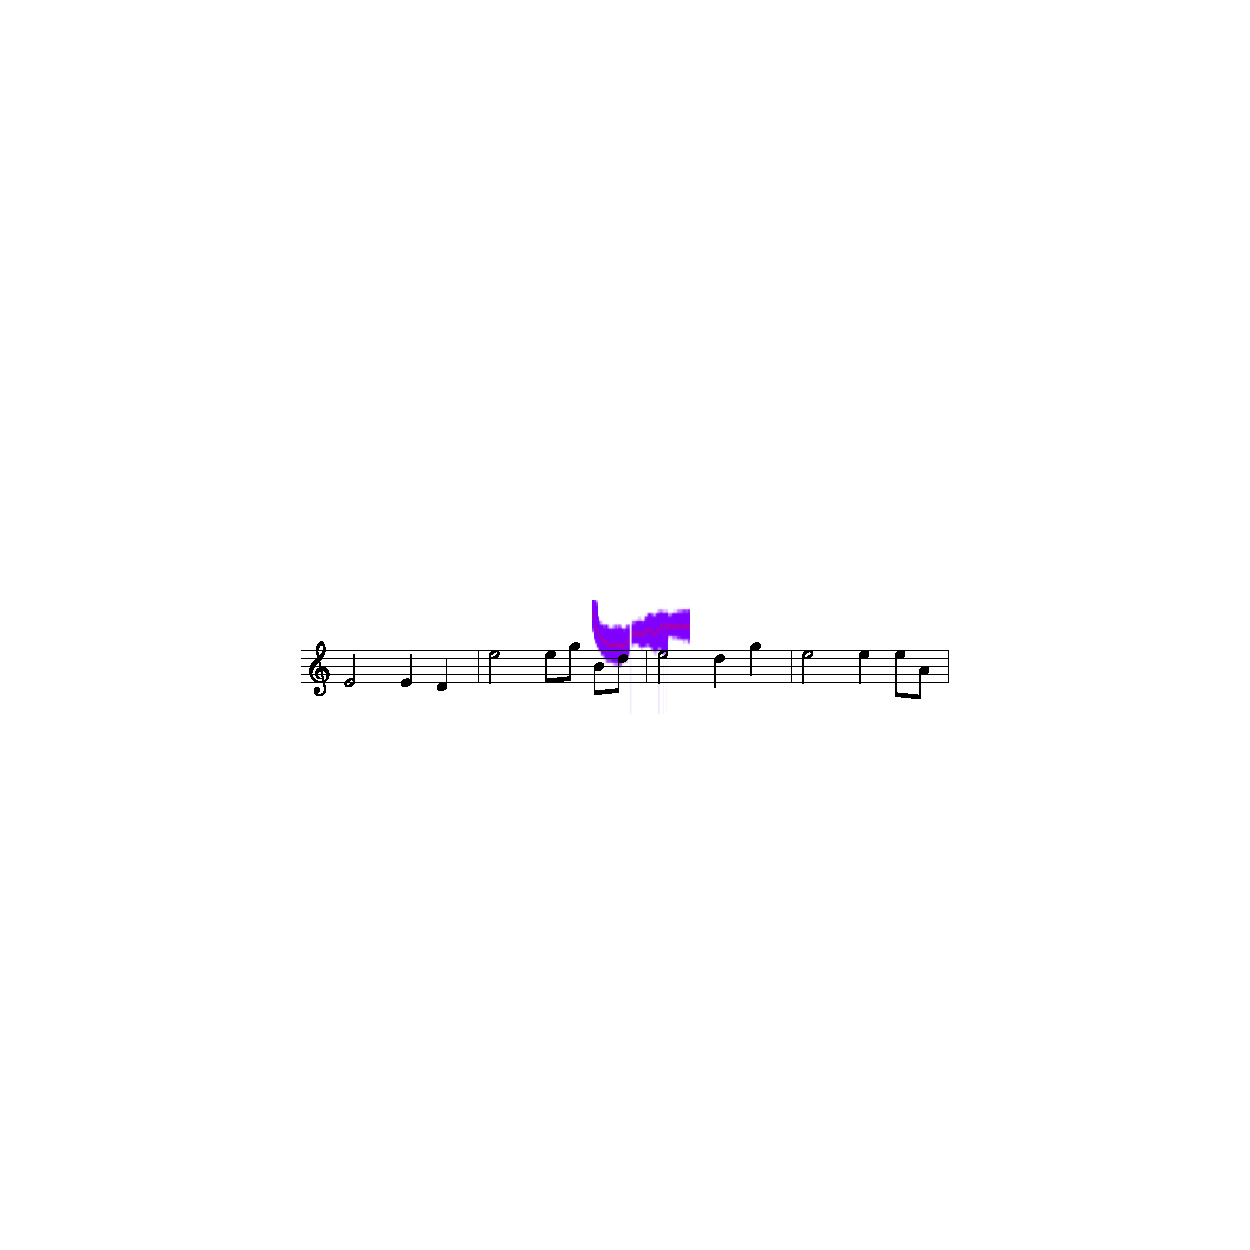
\includegraphics[width=1.6\columnwidth]{imgs/graphsig}}}
\caption{A graphic signal synchronized to a GMN score. The signal can move and receive data in real-time.}
\label{fig:graph}
\end{figure*}


%=============================================================
\section{Conclusion}

Our approach for synchronizing arbitrary objects in the graphic space according to their time relations, combines the advantages of simplicity and flexibility: a great variety of behaviors may be obtained depending on the defined segmentations and mappings. This method is independent of any implementation.

The proposed solution to include the performance representation into the music score is also characterized by its simplicity and flexibility. It consists in abstracting the representation computation from the rendering engine, which results in an opened and dynamically extensible system.

The resulting augmented music score supports heterogeneous components and proposes an original music notation approach, opening new spaces to music and performance representation.

There are many potential application domains, including pedagogic applications, games,... But we also hope that new music forms like interactive music, will take advantage of this research and its developments.

The Interlude Augmented Music Score framework is an open source project. The viewer is available from the Interlude web site at http://interlude.ircam.fr. 



%=============================================================
\vspace{4mm}
\textbf{Acknowledgments} \\
The Interlude project is funded by the Agence Nationale pour la Recherche [ANR-08-CORD-010].


\bibliography{../interlude}

\end{document}
